\subsection{Auf dem Weg zum Raetea Forest}

Auf dem Weg zum Raetea Forest


\begin{figure}[H]
	\centering
	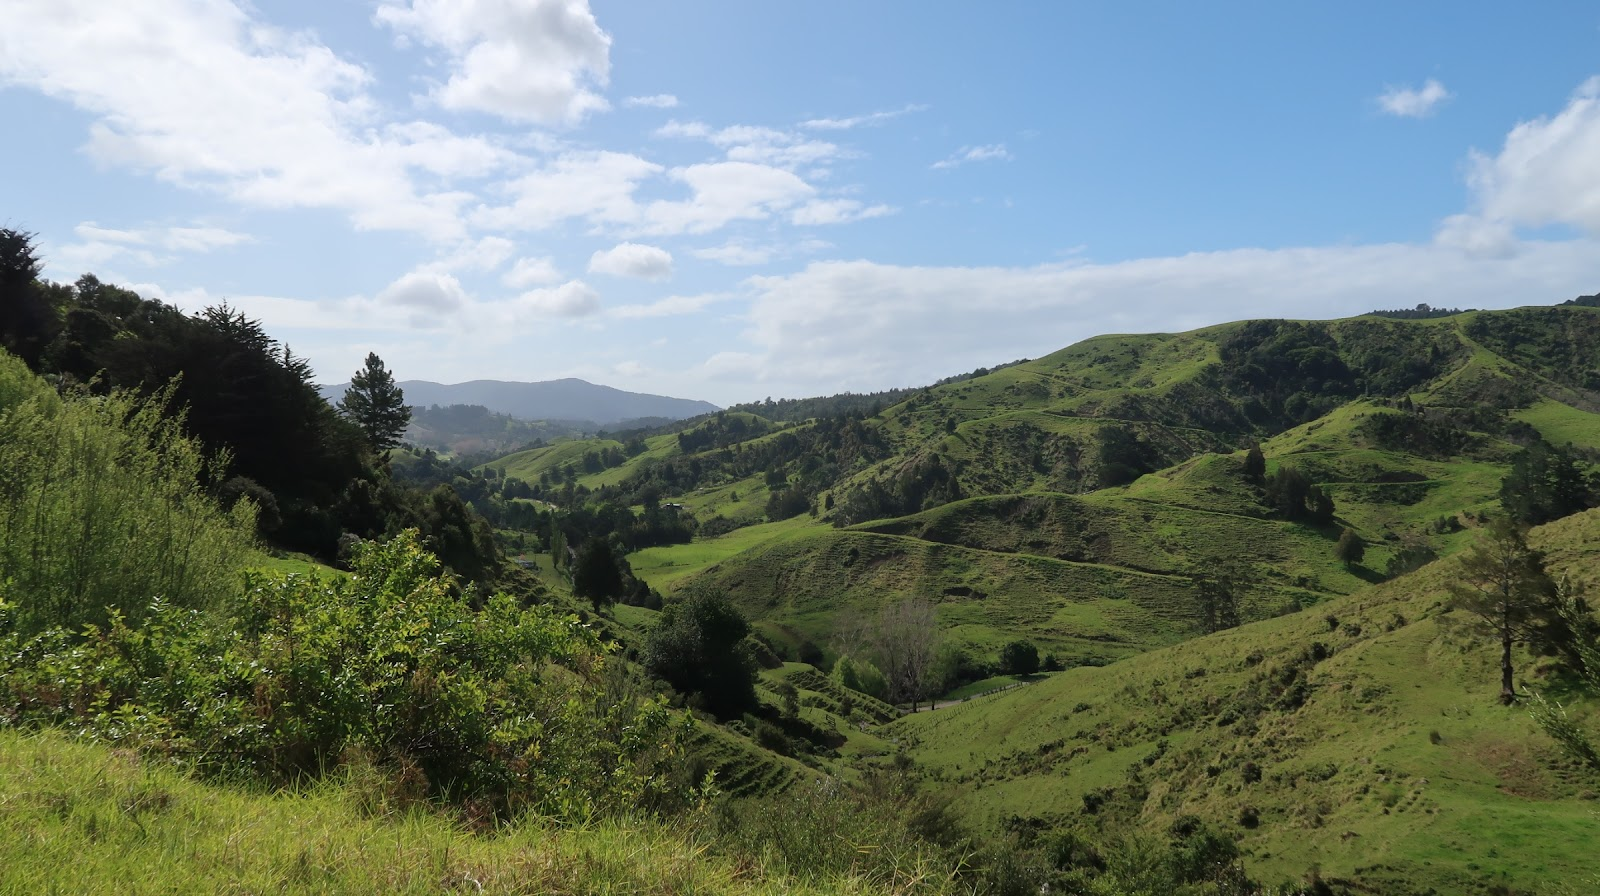
\includegraphics[width=0.5\textwidth]{auf_dem_weg_zum_raetea_forest/10_1666771273444027-0.png}
	\caption{}
	\label{fig:10_1666771273444027-0}
\end{figure}

   SA 22.10.22    Tag 6
  


   Kaitaia - Takahue Saddle Road
  


  Km 115, 6, - 136,7
 


\begin{figure}[H]
	\centering
	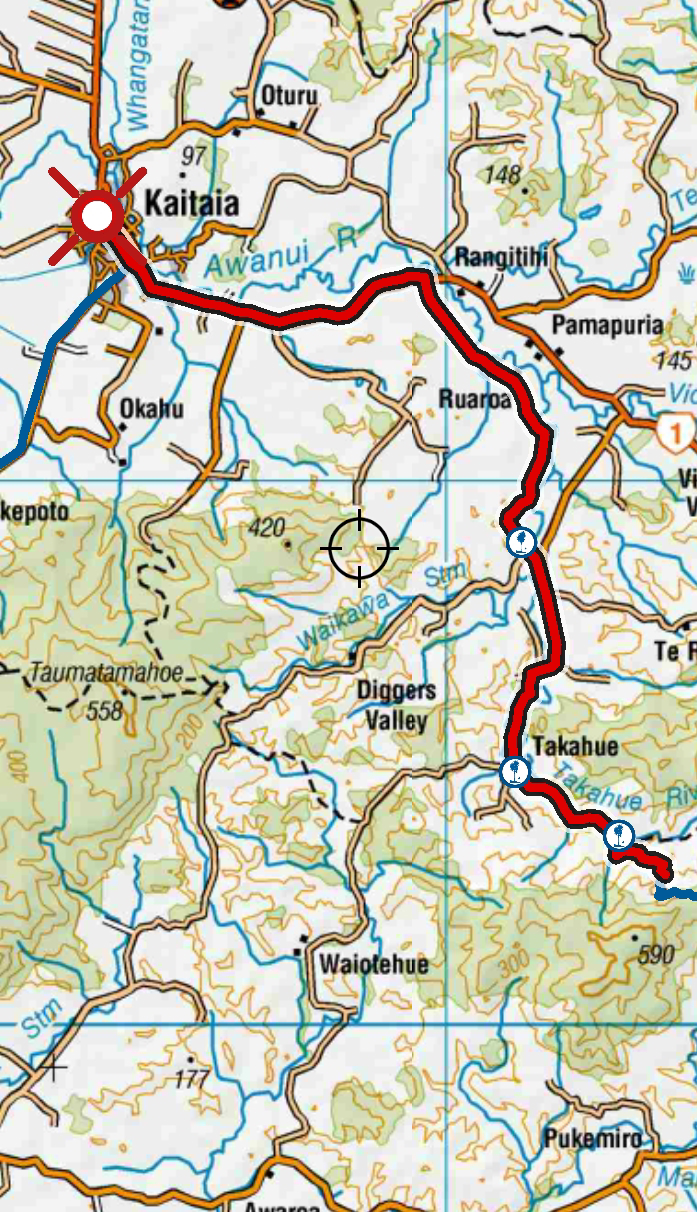
\includegraphics[width=0.5\textwidth]{auf_dem_weg_zum_raetea_forest/11_1666771269406454-1.png}
	\caption{}
	\label{fig:11_1666771269406454-1}
\end{figure}

  Nach einer sehr erholsamen Nacht in einem Motel, mit eigener Toilette und Dusche , (auf dem Zimmer!) und nach einem resupply (=Einkaufen) bei Pack'n Save (Supermarktkette in NZ), für die nächsten 4-5 Tage machen wir uns wieder hochmotiviert auf den Weg.
 


\begin{figure}[H]
	\centering
	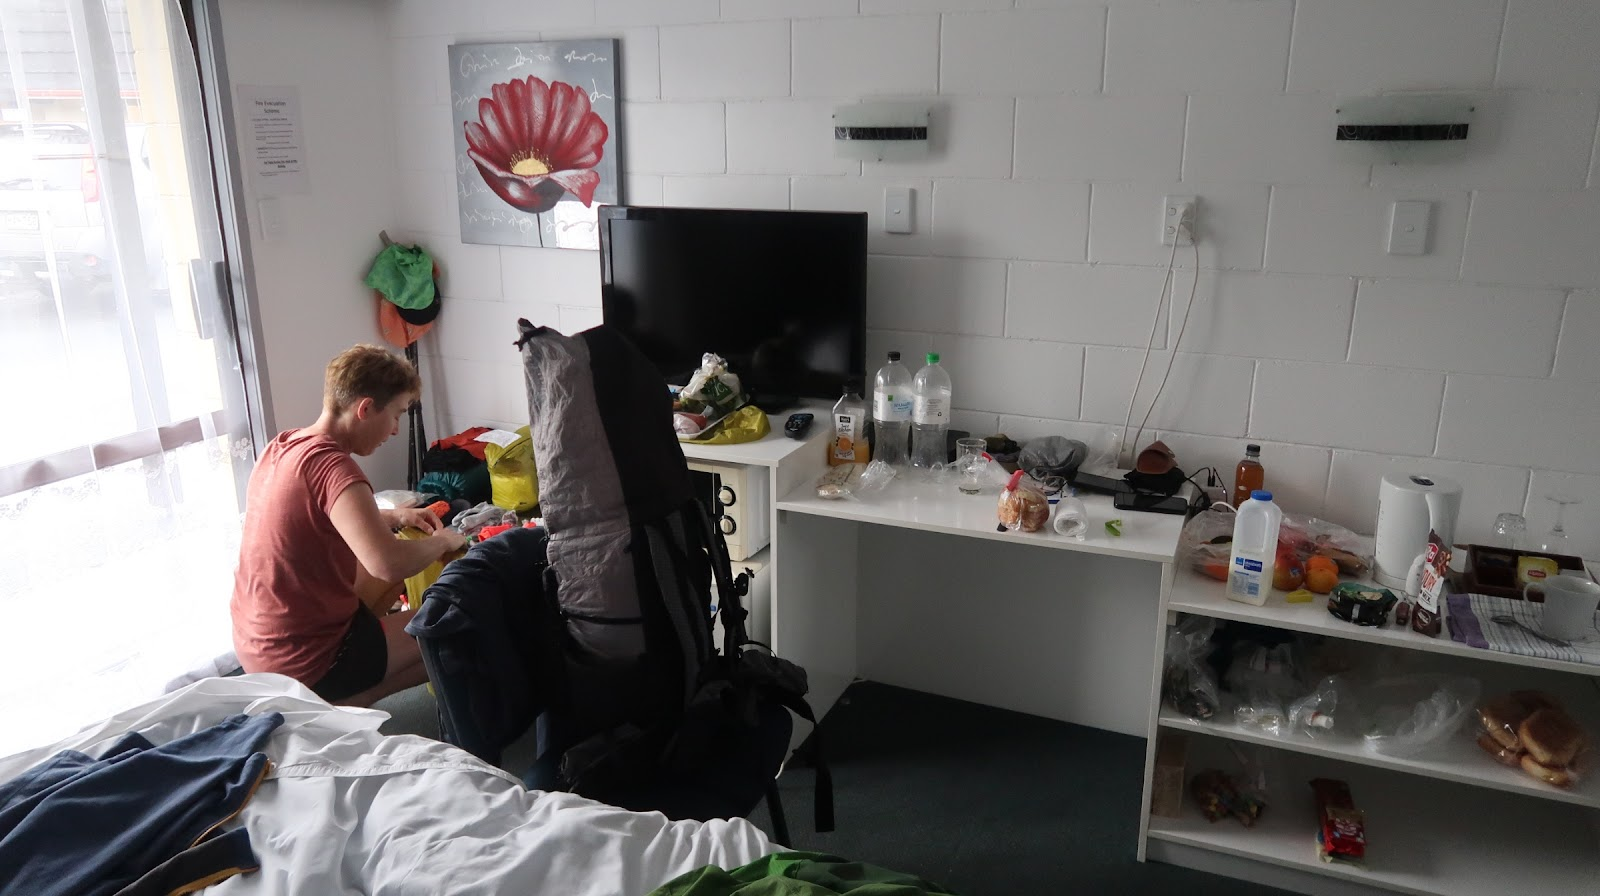
\includegraphics[width=0.5\textwidth]{auf_dem_weg_zum_raetea_forest/12_1666771263644376-2.png}
	\caption{}
	\label{fig:12_1666771263644376-2}
\end{figure}

  Seit mehreren Jahren ist der Weg durch den Herekino Forest, zum Schutz der Kauri Bäume gesperrt. Die Umleitungsstrecke verläuf immer noch entlang des Highway No1 bis Kaitaia. Danach verläuft sie weitere 6 km entlang dem HW 1. Es folgen etwa 11 km auf einer "gravelroad" (Schotterstrasse),  bis nach Takahue. Hier trifft die Umleitungsstecke wieder auf den Orginaltrail.  Die offiziellen Empfehlungen für den HW 1 besagen, man soll es vermeiden ihn zu laufen und irgendwie, z.B. per Anhalter, zu überbrücken. Da unser Plan für dieses Mal einen echten Thruhike vorsieht, gibt es für uns keine Alternative, als zu laufen.
 


  Am Ortsende treffen wir auf Wang, einen jungen chinesischen Mitstreiter mit erhobenen Daumen. Nachdem wir laufen wollen, entscheidet auch er sich für die etwas gefährlichere Variante.
 


\begin{figure}[H]
	\centering
	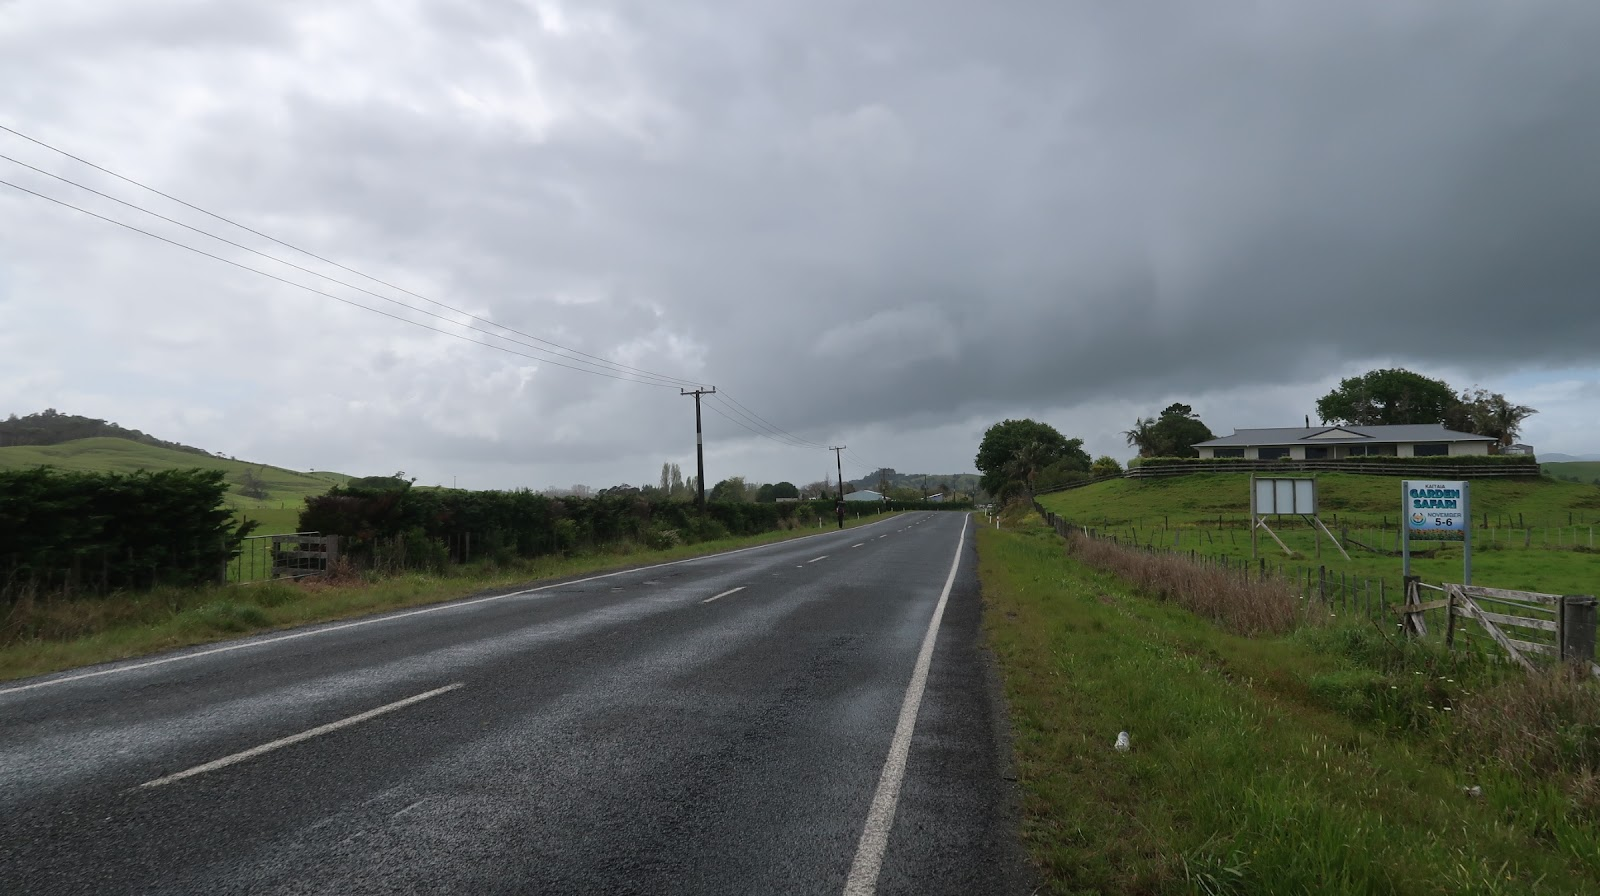
\includegraphics[width=0.5\textwidth]{auf_dem_weg_zum_raetea_forest/13_1666771258775532-3.png}
	\caption{}
	\label{fig:13_1666771258775532-3}
\end{figure}

  Heute ist jedoch nicht sehr viel Verkehr und wir schaffen auch die nächsten 6 Kilometer unbeschadet, bis zur Abzweigung nach Takahue. Lediglich mehrere Hunde am Straßenrand machen uns das Leben  schwer, hier könnte sich Martin Rütter ( TV- Hundtrainer) mal so richtig verausgaben. Bis nach Takahue verläuft der Weg ohne große Störungen, wenn man von den vier angehenden Motocross Stars einmal absieht, die diese Schotterpiste als Trainingsstrecke nutzen  und ständig aus verschiedenen Richtungen an uns vorbei rasen.
 


\begin{figure}[H]
	\centering
	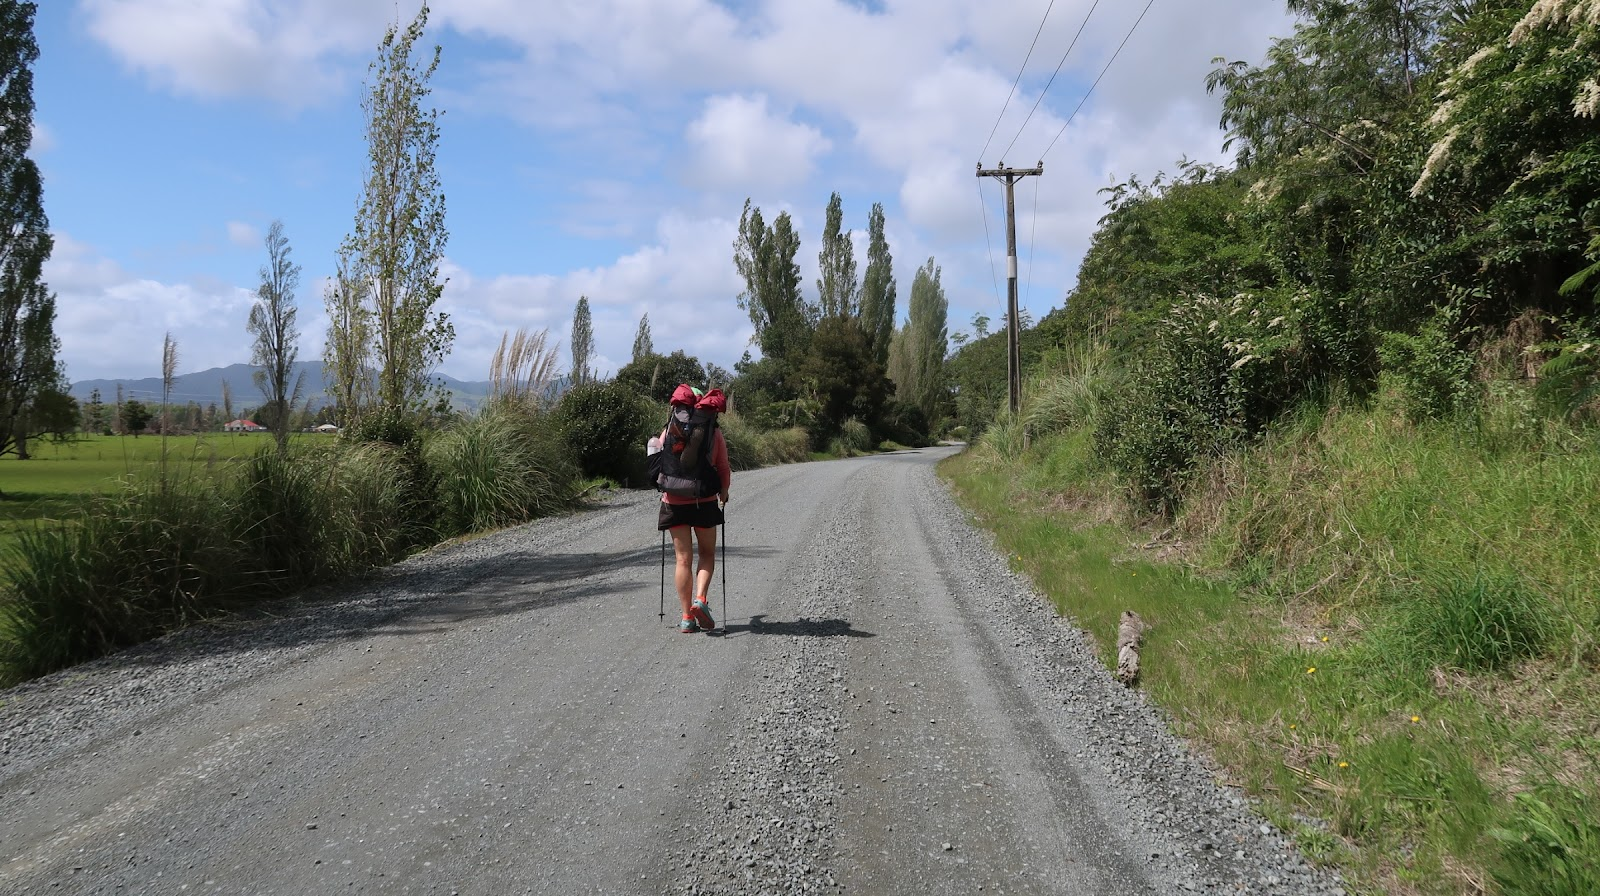
\includegraphics[width=0.5\textwidth]{auf_dem_weg_zum_raetea_forest/14_1666771251663002-4.png}
	\caption{}
	\label{fig:14_1666771251663002-4}
\end{figure}

\begin{figure}[H]
	\centering
	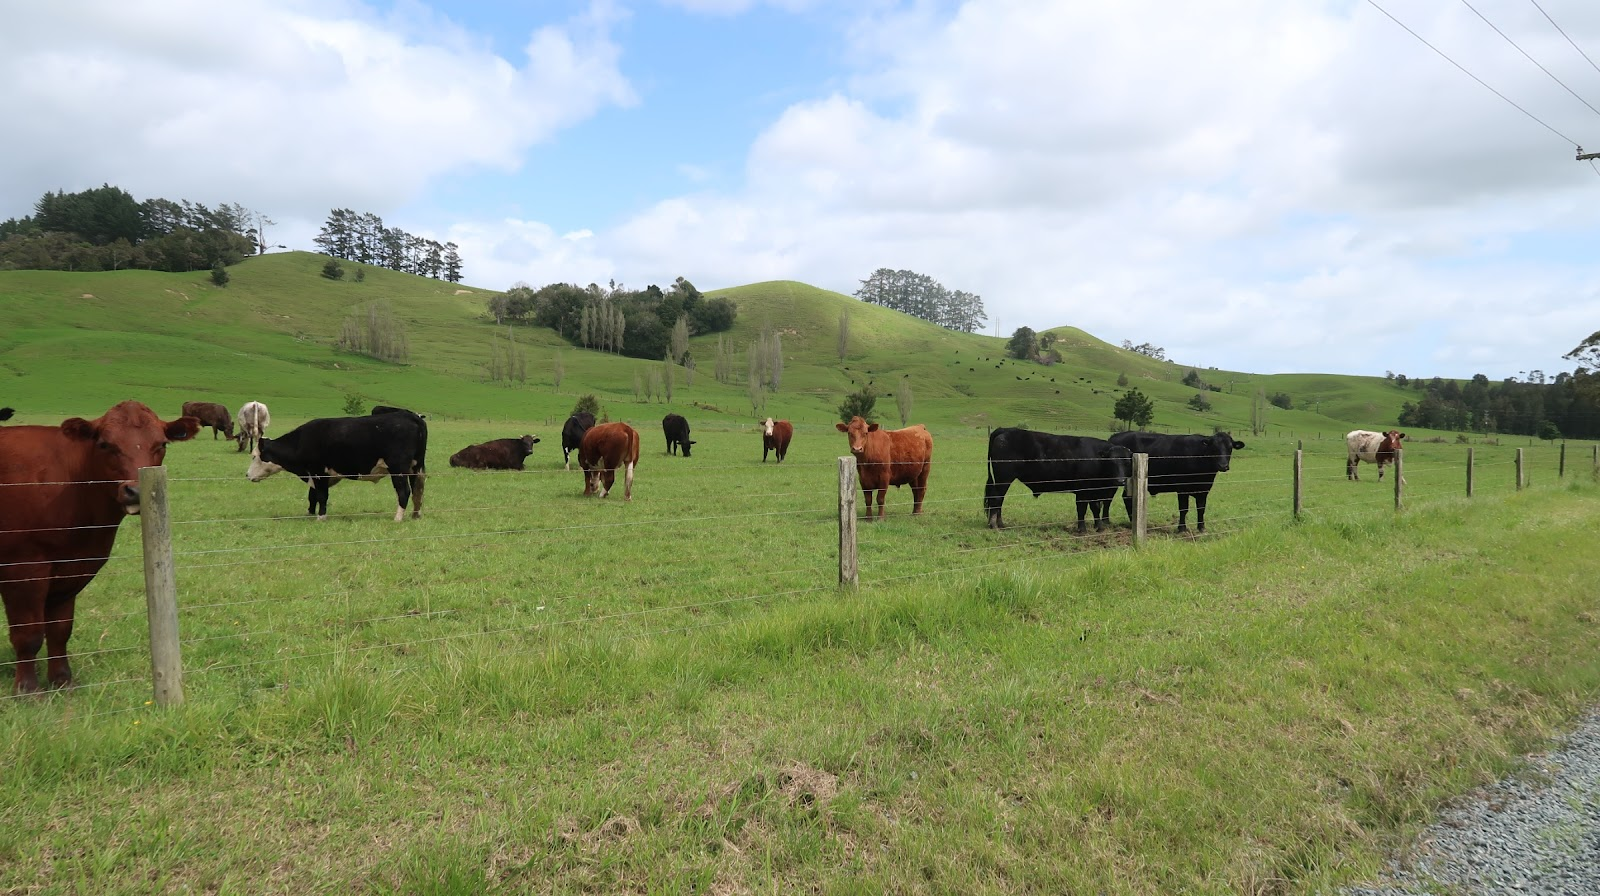
\includegraphics[width=0.5\textwidth]{auf_dem_weg_zum_raetea_forest/15_1666771246496971-5.png}
	\caption{}
	\label{fig:15_1666771246496971-5}
\end{figure}

  Schließlich erreichen wir irgendwann die Takahue Hall, eine kleine Veranstaltungshalle im Nirgendwo.
 


\begin{figure}[H]
	\centering
	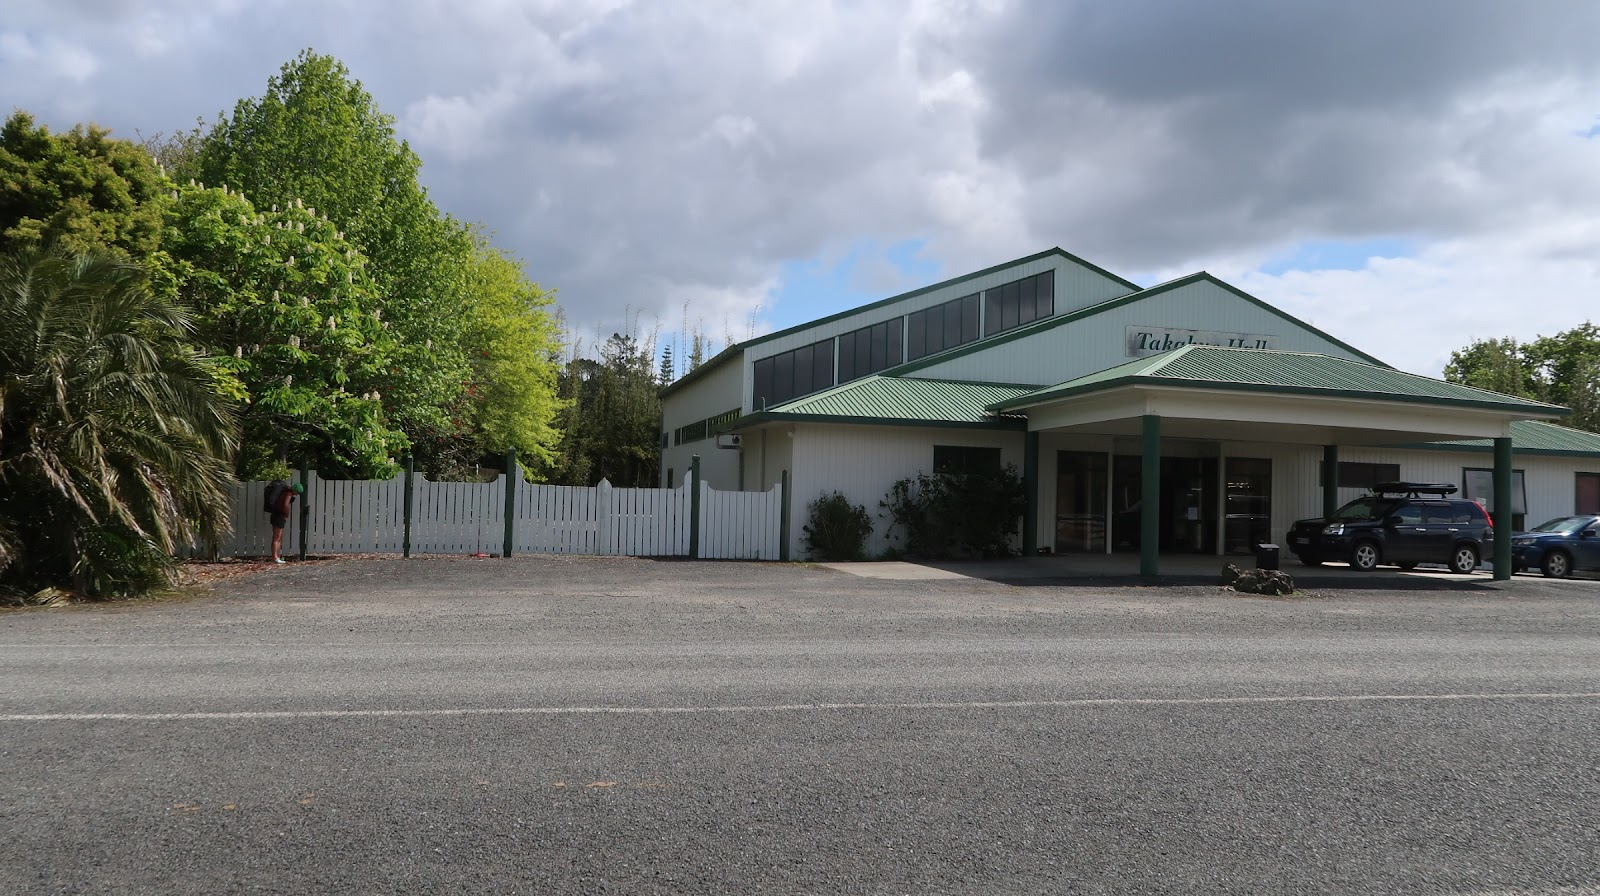
\includegraphics[width=0.5\textwidth]{auf_dem_weg_zum_raetea_forest/16_1666771241241663-6.png}
	\caption{}
	\label{fig:16_1666771241241663-6}
\end{figure}

  Nachdem die Tür geöffnet ist, will ich kurz nachfragen, ob wir die Toilette benutzen dürfen. Ich folge den Stimmen bis zur Küche. Hier treffe ich auf fürchterliche Dinge, zumindest für einen Long Distance Hiker, nämlich Essen. Essen das gerade für eine Hochzeit gerichtet wird, etwa 2 m lange Rollbraten werden für den Grill vorbereitet, Kartoffeln und Salate werden gerichtet....
 


\begin{figure}[H]
	\centering
	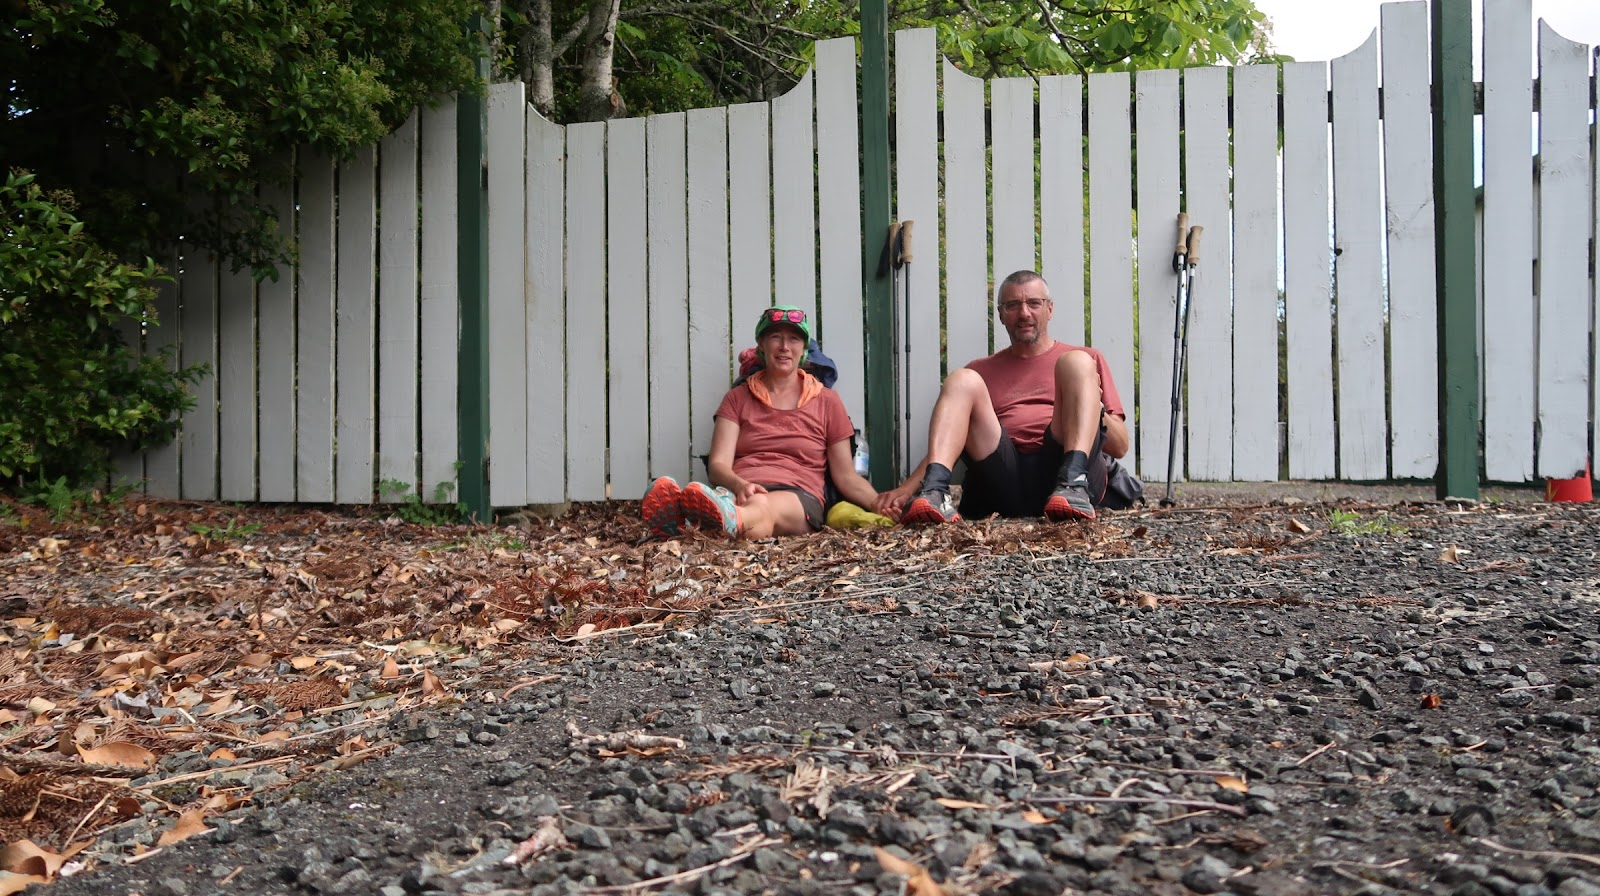
\includegraphics[width=0.5\textwidth]{auf_dem_weg_zum_raetea_forest/17_1666771235664149-7.png}
	\caption{}
	\label{fig:17_1666771235664149-7}
\end{figure}

  Jetzt sind es nur noch etwa 5 km bis zu einem kleinen privat angelegten Camp, hier waren wir schon vor 4 Jahren zu "Gast" .
 


\begin{figure}[H]
	\centering
	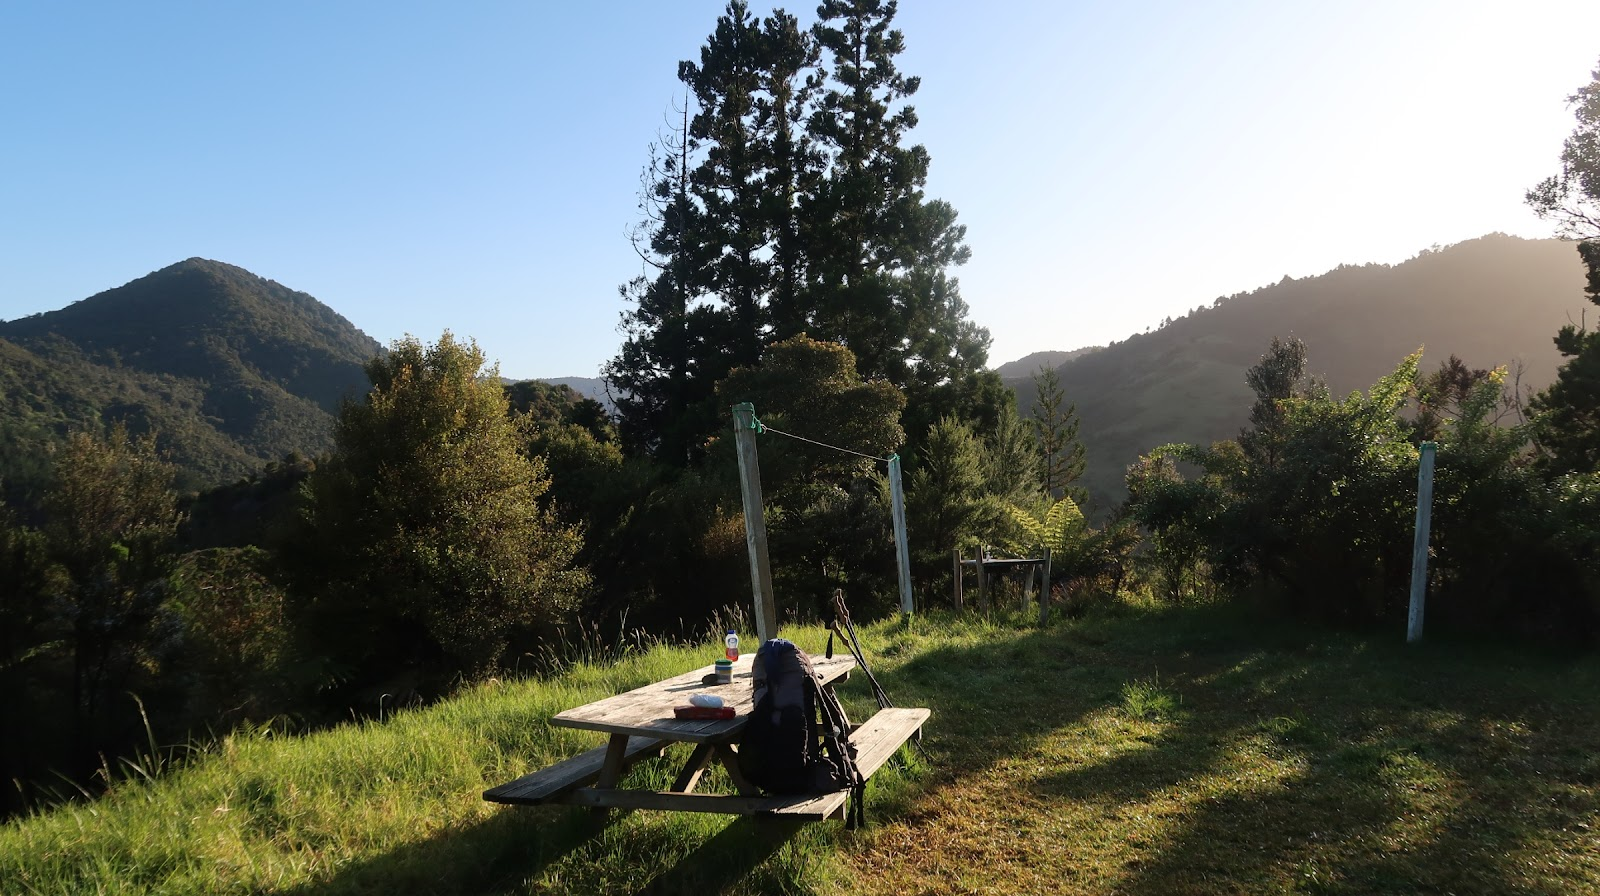
\includegraphics[width=0.5\textwidth]{auf_dem_weg_zum_raetea_forest/18_1666771230022596-8.png}
	\caption{}
	\label{fig:18_1666771230022596-8}
\end{figure}

  Es gibt mittlerweile einen Tisch mit Bänken, einen Regenwassertank und eine Toilette. Die Toilette besteht eigentlich nur aus einem Loch mit einem Holzdeckel auf der Erde, deren Füllstand schon fast den Deckel erreicht hat.
 


  Macht uns nichts aus, besser als gar nichts, dafür haben wir einen tollen Ausblick.
 


\begin{figure}[H]
	\centering
	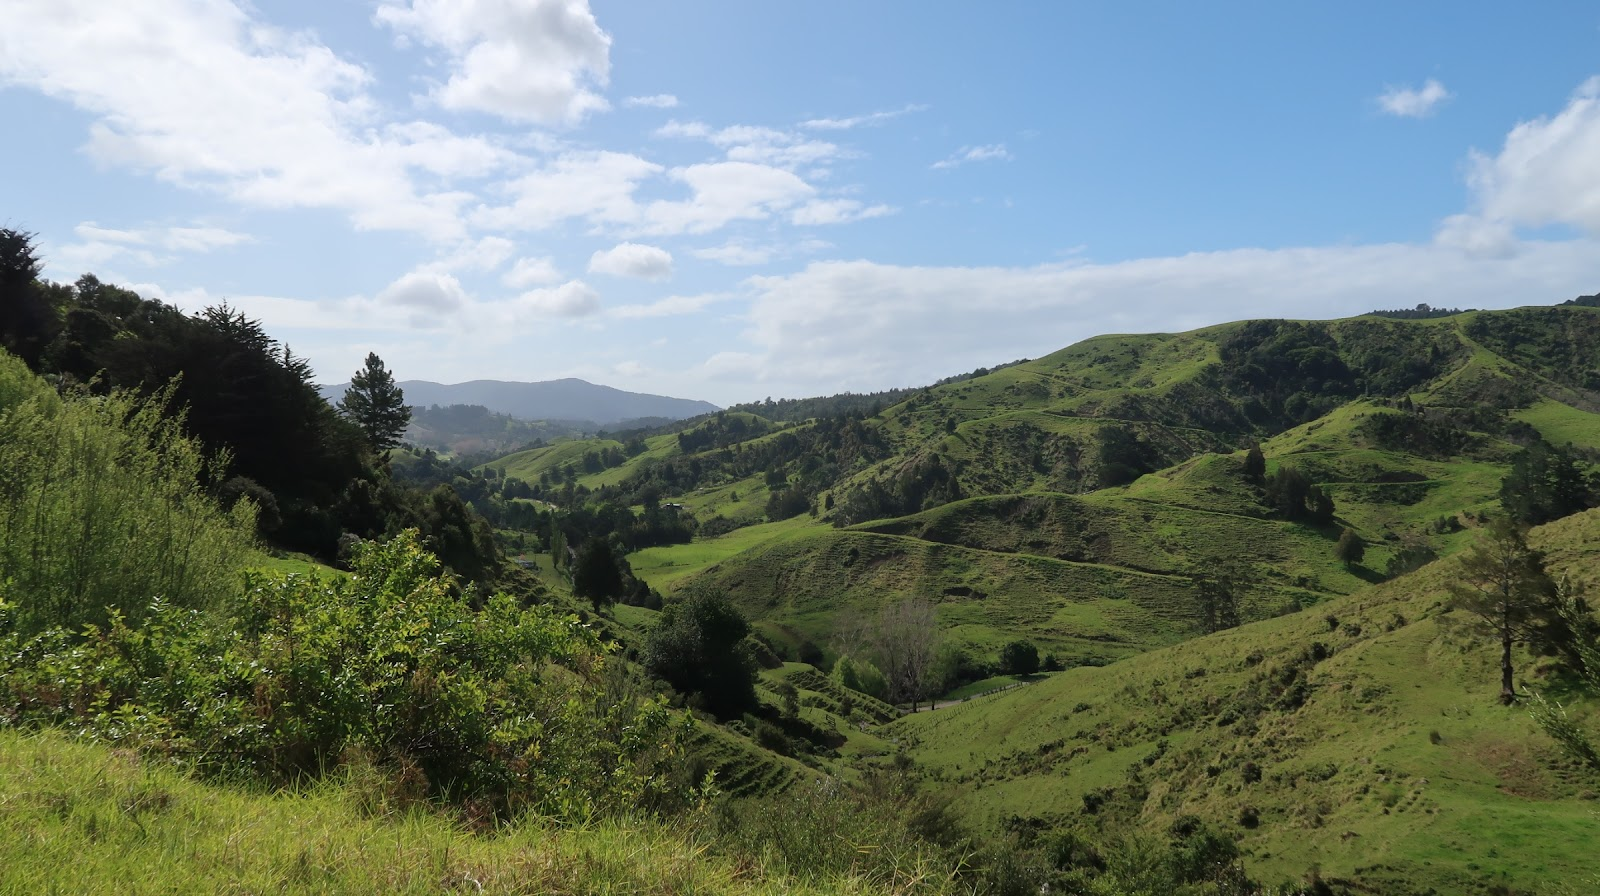
\includegraphics[width=0.5\textwidth]{auf_dem_weg_zum_raetea_forest/19_1666771224561329-9.png}
	\caption{}
	\label{fig:19_1666771224561329-9}
\end{figure}

  Morgen steht  mit dem Raetea Forest vielleicht eine der schwierigsten Etappen der Nordinsel, auf dem Programm.  Diese ist offiziell eigentlich, nach einem Unwetter, mit unzähligen umgestürzten Bäumen und ein paar Hangabrutschungen noch gesperrt. Es gibt hier einen eher langweiligen Plan B. Zunächst dem normalen noch befahrbaren Weg hinauf bis zum Takahue Saddle, danach auf dem Fahrweg hinunter nach Broadwood, von dort bis zur Straße
 


  nach Mangamuka um hier auf den Orginaltrail zu treffen. Jetzt geht's erst mal ins Bett und morgen schauen wir weiter.
 


  gelaufenen 21,1 km
 


  Wir erwarten von unseren Lesern übrigens , dass sie die angegebenen Orte alle irgendwie nachverfolgen. 
 

